\documentclass[a4paper]{article}

\usepackage[english]{babel}
\usepackage[utf8]{inputenc}
\usepackage{amsmath}
\usepackage{graphicx}
\usepackage[colorinlistoftodos]{todonotes}
\usepackage{pdfpages}
\usepackage{listings}

\title{InfoEmb TP2}

\author{Jérôme Skoda}

\date{\today}

\begin{document}
\maketitle

\begin{abstract}
 Colimaçon: \newline
 001  002  003  004  005  006  007  008  009  010 \newline
 022  023  024  025  026  027  028  029  030  011 \newline
 021  020  019  018  017  016  015  014  013  012 \newline
\end{abstract}

\section{Comment compiler le projet}

\begin{itemize}
\item make all: Compile tout les fichiers
\item make test: Lancement de la série de tests automatiques
\item make lib: Génération de la bibliothéque static et dynamique
\item make doc: Génération de la documentation (doxygen)
\item make rapport: Génération du rapport (latex)
\item make clean: Nettoyage du projet (supression des objets et binaires)
\item make demo-1 ligne=X col=X: Lancer la démo colimacon
\item make demo-2: Lancer la démo horizontal
\item make demo-3: Lancer la démo vertical
\item make demo-4: Lancer la démo carré
\item make demo-5 ligne=X col=X: Lancer la démo colimacon sans print (utile pour le bench)
\item make demo-6 ligne=X col=X: Lancer la démo colimacon avec sortie temps (utile pour le bench)
\end{itemize}

\section{Arborescence}

\begin{itemize}
\item bin : Binaire exécutable
\begin{itemize}
  \item demo : Exécutable de démonstration
  \item test : Exécutable de test
\end{itemize}
\item lib : Bibliothéque
\item doc : Documentation doxygen sous differents formats
\item rapport : Source du rapport
\item res : Ressources necessaire au projet (fichier de bdd)
\item script  : Script utilisé pour les test
\item src : Source du projet
\begin{itemize}
  \item colimacon : Source de colimacon
  \item demo  : Sources des differentes démonstrations d'utilisation
  \item test  : Sources des dufferents tests
\end{itemize}

\item sujet.pdf  : Sujet du projet
\item README.md  : Le readme du projet
\item rappot.pdf : C'est moi
\end{itemize}

\section{Test disponible}
Les test fonctione de la manière suivante: un script bash exécute chacun de binaire de
test un par un en enregistrant le sortie standard dans un fichier .out
Ensuite il compare avec la commande diff chacun des fichier .out avec la
valeur attendu dont la valeur est stoqué dans un fichier .expected

Les fichier .out et .expected sont dans le répertoire src/test/
Le script se situe dans le repertoire script

Les test disponible sont:
\begin{itemize}
  \item  colimacon 1x1
  \item  colimacon 1x10
  \item  colimacon 10x1
  \item  colimacon 10x2
  \item  colimacon 2x10
  \item  colimacon 10x10
  \item  colimacon 1000x1000 (sans print)
\end{itemize}


\section{Fonctionnement}

Le remplissage s'effectue avec un systeme de borne (voir struct borne) et de séquence de direction (voir direction\_t).
Chacune des écriture sont faite dans un ordre de direction: DROITE puis BAS puis GAUCHE puis HAUT jusqu'à que le tableau soit remplis.
L'écriture dans une direction fonctionne de cette manière suivante:
\begin{itemize}
  \item On calcule la position inital du curseur en fonction des borne et de la direction. (\_get\_position\_initiale)
  \item On regarde si l'on peux ecrire dans la case calculé (\_canWrite)
  \item S'il est possible d'écrire, on le fait puis on réitére l'operation en avançant le curseur d'une case à chaque fois (\_iter\_curseur)
  \item Enfin quand l'écriture n'est plus possible, on avance la borne en fonction de la direction d'écriture (\_iter\_borne) et l'on passe à la direction suivante
\end{itemize}
Voici une petite illustration:

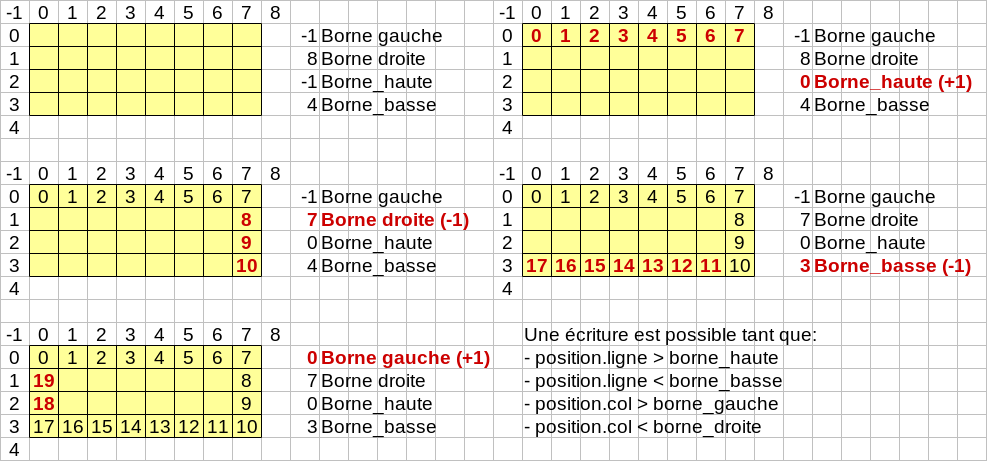
\includegraphics[width=0.8\textwidth]{exemple.png}


\section{Estimation du temps}

J'ai estimé la réalisation en une journée (environs 7h-12h). Je me suis un peu
surestimé, il m'a fallu une demi-journée en plus.

Concernant la partie codage (sans compter la doc), d'après l'historique de
mon dépôt, j'estime le temps réellement passé sur le 1h sur colimacon.c et
une 30taine de minutes sur les demos et tests.

Tout le reste est essentiellement passé dans toutes les fonctionnalité:
makefile, doc, bench, rapport plein de fautes, schéma dégeux sur excel, latex
qui dégénère et les sympathiques ifndef de makefile qui ne doivent pas être
indenté dans les rules.

\section{Choix et problémes}

\begin{itemize}
  \item Bien nommer les choses, ce n'est parfois pas évidant. Exemple:
    avec un tableau 3x3: les valeurs lors de l'initilisation
    des bornes sont: borne haute= -1 et borne basse=3 ça peux preter confusion
    car haute\textless basse.
  \item Le script de test, j'en suis particuliérmeent fière, je le resort à
    chaque fois en projet de c. C'est un simple foreach sur chaque executable
    de test avec la sortie standard redirigé vers un .out et procéde à un diff
    sur le .expected.
  \item J'ai eu des problémes à comprendre comment utiliser perf.
  \item Le travaille de relecture... Parler à des gens quelle horreur!
\end{itemize}


\section{Prototype}

Mon prototype:
\begin{lstlisting}[frame=single]
int ** colimacon(int line, int col);

void delete_colimacon(int** table, int line, int col);
\end{lstlisting}

L'avantage est que la fonction d'occupe de
l'allocation memoire, il n'y a donc pas de risque de l'utilisateur passe
un tableau avec le nombre de ligne ou colonne qui ne correspondent pas.
Le defaut est que du coup, pour le delete, il y a besoin du nombre
de ligne et de colonnes.

\begin{lstlisting}[frame=single]
int colimacon (int ** tab, int line, int col)
\end{lstlisting}

Ce propotype est interessant car il permet de retourné une erreur par exemple.

\section{Paralelisation}

Le programme n'est pas dutout parralelisable, cependant avec quelques
modification il est possible de le rendre sur chacune des directions.

Il faudra cependant modifier quelques functions:
\begin{lstlisting}[frame=single]
static int _ecriture_direction(int** tab, struct borne* bor, int* val,
  direction_t dir)
\end{lstlisting}
Devras travailler avec une bornes et un valeur en copie ce qui donnera:
\begin{lstlisting}[frame=single]
static int _ecriture_direction(int** tab, struct borne bor, int val,
  direction_t dir)
\end{lstlisting}

Il faudra ajouter un fonction qui calcule l'incrementation des valeurs après
chaque direction. Par exemple:
\begin{lstlisting}[frame=single]
int _iter_val(struct borne bor, direction_t dir)
\end{lstlisting}

Enfin dans la boucle de colimacon:

\begin{lstlisting}[frame=single]
  while(1) {

    a lancer sur le thread 1:
    _ecriture_direction(table, borne, valeur, DROITE)

    valeur= _iter_val(bor, DROITE)
    _iter_borne(bor, DROITE)

    a lancer sur le thread 2:
    _ecriture_direction(table, borne, valeur, BAS)

    valeur= _iter_val(bor, BAS)
    _iter_borne(bor, BAS)

    [...]
  }
\end{lstlisting}

Le crois qu'il faudra aussi faire de l'allocation en mémoire partagée.
Globalement l'idée de l'algorithme est compatible avec une paralelisation.

Cependant, il ne sera pas possible de remplir chaqu'une des cellules en
parallèle, car il faudrait trouver un autre mécanisme que celui du curseur
qui se déplace vers une direction.

Pour conclure:
Ecrire plusieurs rangée complete du tableau c'est possible en
gardant la logique de l'algorithme
Ecrire chacune des cellule du tableau ce n'est pas possible avec la logique de
l'algorithme.

Remarque: Je ne vois pas trop l'intrêt de paralleliser toutes les cases car
les mécanismes d'enregistrement et lancement de thread risque d'avoir une
performance médiocre.

\section{Temps d'execution}

La mesure s'est effectué avec la commande make bench [nombre-d'échantillon]
[fichier de sortie]

Cette commande lance le script/bench.sh qui consite à faire la moyenne du temps
d'execution de bin/demo/6-colimacon-no-print sur n échantillons et ce sur
differente taille.

Voici le resultat sur 1 000 échantillons:

\begin{tabular}{|l|l|l|}
  \hline
  Taille & Laptop & Desktop \\
  \hline
  10x10 & 0.035371 ms & 0.021329 ms\\
  \hline
  100x100 & 0.209286 ms & 0.112920 ms \\
  \hline
  1000x1000 & 15.301931 ms & 7.218361ms \\
  \hline
  10000x10000 & 1.513250620s & .989898073s \\
  \hline
\end{tabular}


\begin{itemize}
  \item Laptop:
    \begin{itemize}
      \item CPU: i5-2430M CPU @ 2.40GHz 2 cores 4 threads
      \item RAM: 16Go @ 1 600MHz
    \end{itemize}
  \item Desktop:
    \begin{itemize}
      \item CPU: i7 4790K @ 4.3GHz 4 cores 8 threads
      \item RAM: 32Go @ 1 600MHz
    \end{itemize}
\end{itemize}

\section{Accès mémoire}

\begin{lstlisting}[frame=single]
int ** colimacon(int line, int col);
\end{lstlisting}

Cette fonction accède 0 fois au tableau en lecture et N fois en écriture.

\begin{lstlisting}[frame=single]
void print_colimacon(int** table, int line, int col);
\end{lstlisting}

Cette fonction accède N fois au tableau en lecture et 0 fois en écriture.

\section{Occupation mémoire}

Sur le profilage de bin/test/7-1000x1000, on remarque que la plupart des écritures
memoire s'effectue dans le cache L1 et qu'il n'y pas
enormément de latance (3.85%).

Concenrnat la lecture, la fonction \_can\_write a le plus de latance
(11.29\% et 6.53\%) et utilise la pile.

\_get\_position\_initiale utilise la pile
\_ecritrue\_direction utilise le tas.

Petit memo:
\begin{lstlisting}[frame=single]
sudo perf mem record bin/test/7-1000x1000
sudo perf mem report
\end{lstlisting}

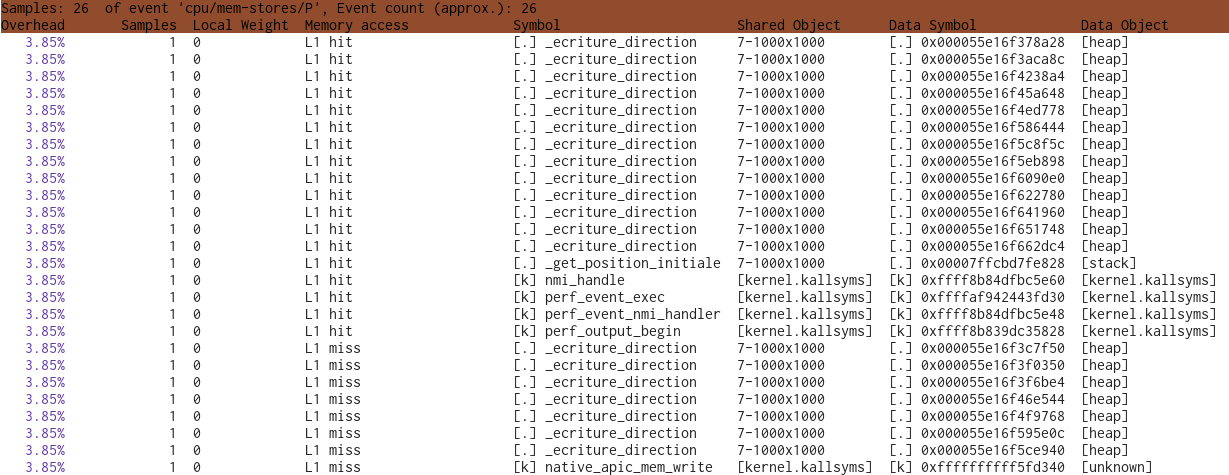
\includegraphics[width=1\textwidth]{mem-store-revert.png}

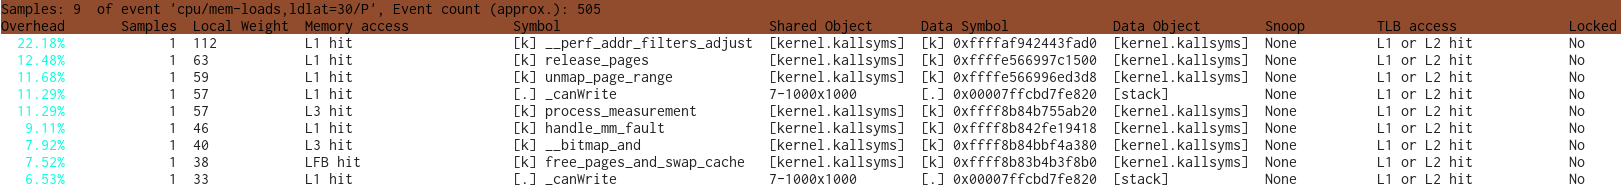
\includegraphics[width=1\textwidth]{mem-loads-revert.png}


\section{Relecture}

Liang m'a dit qu'ils n'ont rien compris au code. Du coups, j'ai augmenté la documentation.
Li Xiang m'a dit j'ai fait la même chose que lui sauf que mes fonctions auxilaire rendais le tout plus structuré.

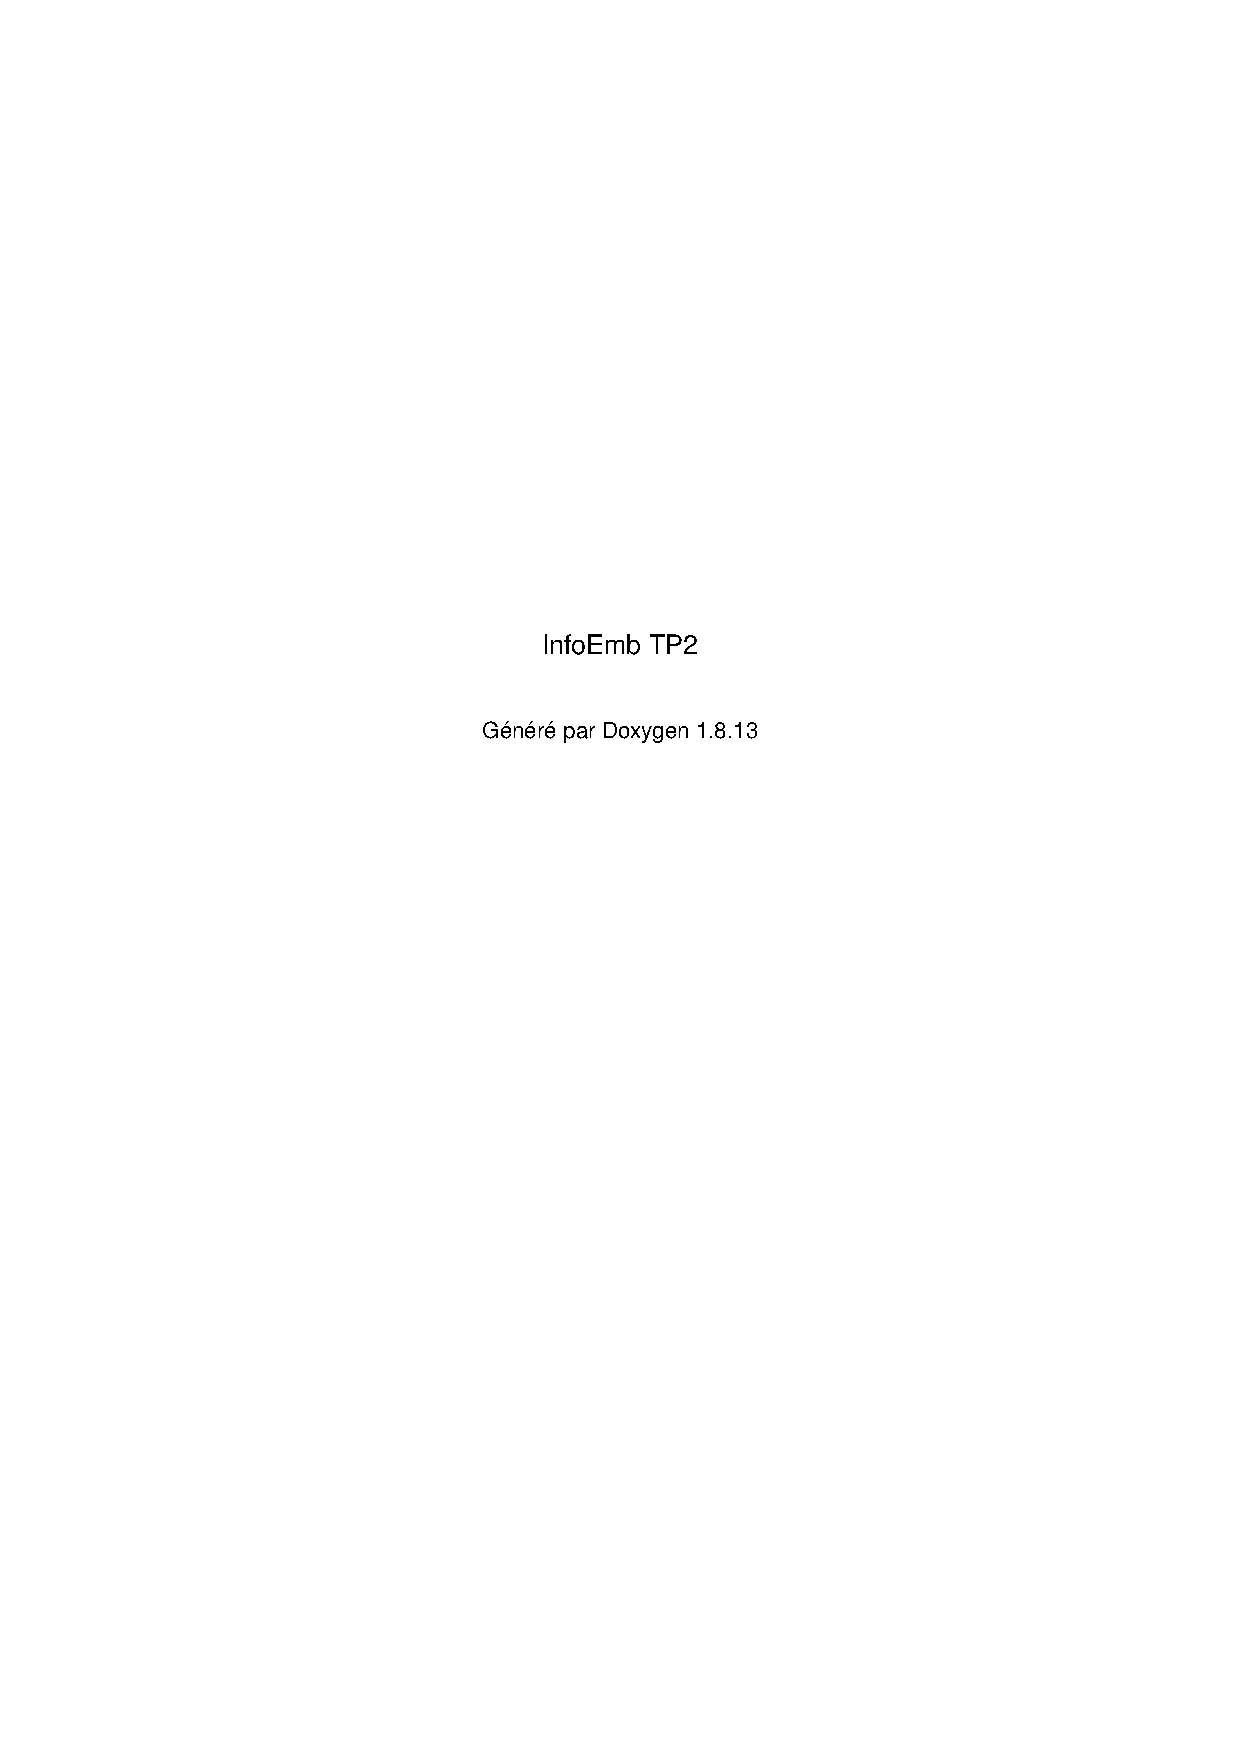
\includepdf[pages=1-15]{refman.pdf}

\end{document}

